% -*- latex -*-
%%%%%%%%%%%%%%%%%%%%%%%%%%%%%%%%%%%%%%%%%%%%%%%%%%%%%%%%%%%%%%%%
%%%%%%%%%%%%%%%%%%%%%%%%%%%%%%%%%%%%%%%%%%%%%%%%%%%%%%%%%%%%%%%%
%%%%
%%%% This text file is part of the source of 
%%%% 'Parallel techniques'
%%%% by Ángel de Vicente, copyright 2019
%%%%
%%%% TO DO:
%%%%
%%%% intermediate-fortran.tex : intermediate fortran towards a
%%%%      Barnes-Hut N-body implementation
%%%% 
%%%%%%%%%%%%%%%%%%%%%%%%%%%%%%%%%%%%%%%%%%%%%%%%%%%%%%%%%%%%%%%%
%%%%%%%%%%%%%%%%%%%%%%%%%%%%%%%%%%%%%%%%%%%%%%%%%%%%%%%%%%%%%%%%

\Level 0 {Intermediate Fortran}
\label{sec:intermediate-fortran}

In order to implement the Barnes-Hut algorithm described in chapter
\ref{ch:barnes-hut.tex} we will need to learn some intermediate programming
concepts.

\Level 1 {Procedures and recursion}
\includepdf[frame=true,scale=0.98,pages={2-12,18-19}]{graphics/procedures_recursivity.pdf}
       
\Level 1 {Pointers and derived types}
{\includepdf[frame=true,scale=0.98,pages={2-21}]{graphics/pointers_derived_types.pdf}}




